\selectlanguage{english}
\def\<#1>{\textit{#1}}

\chapter{FIFO Queues}
\section{Introduction}

FIFO Queues are one of the most widely used data structures. They have been studied thoroughly and are used in many projects. Applications of queues range from web servers to interruption managing, inter-process communication, CPU schedulers and many more. They are essential on any application that requires some sort of First in First out ordering of data.

Queues are usually implemented by linked lists and support two simple operations; enqueue and dequeue, shown in figure \ref{basic_enqueue} and \ref{basic_dequeue}


\begin{figure}
 \centering
  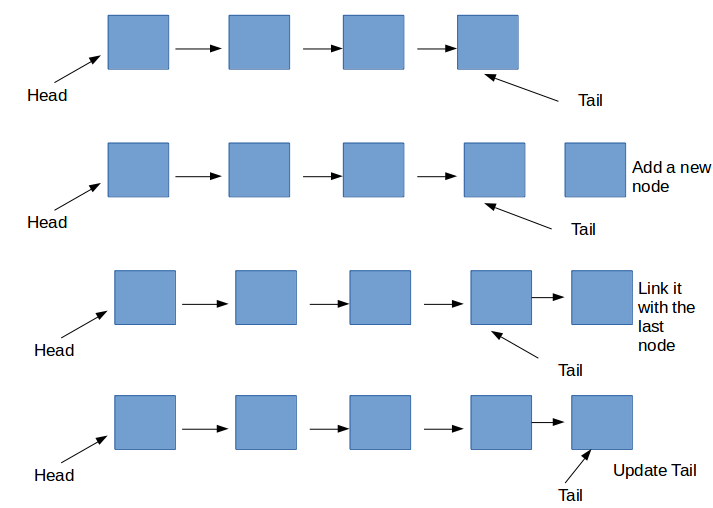
\includegraphics[scale=0.5]{basic_enqueue.png}
\caption{ The basic enqueue operation}
\label{basic_enqueue}
\end{figure}

\begin{figure}
 \centering
  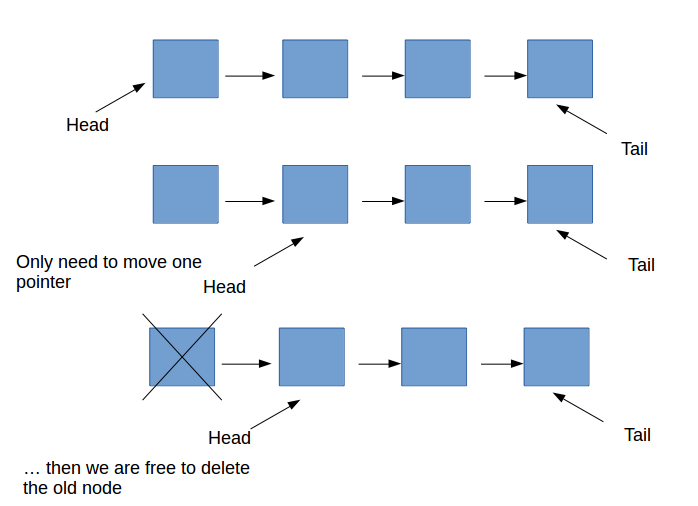
\includegraphics[scale=0.5]{basic_dequeue.png}
\caption{ The basic dequeue operation}
\label{basic_dequeue}
\end{figure}

In many applications, there is the need of having multiple threads, communicating through a shared queue, that is often needed to serve millions of operations per second. Concurrent queues can be quite handy in a scenario where multiple producer threads create work items, that need to be consumed by several worker threads. Producers may create many items in a burst, while consumer threads are receiving them at a slower rate, so the excess of times need to be organized in an efficient manner. Although situations like that can be quite common, implementing an efficient queue that allows concurrent access from multiple threads can be quite challenging. For this reason, concurrent FIFO Queue implementations attract theoretical, as well as practical interest. 
 
In order to maintain the coherence of the data structure in a multi-threaded environment, synchronization between threads is needed. An example of what could go wrong without proper synchronization is shown in figure \ref{queue_no_sync} .Queues are a structure that, by its nature, allows low levels of concurrency, since all reads and writes are applied on Head and Tail, rendering these locations as hot-spots. Therefore, we expect low scalability, as the number of parallel threads increases.

\begin{figure}
 \centering
  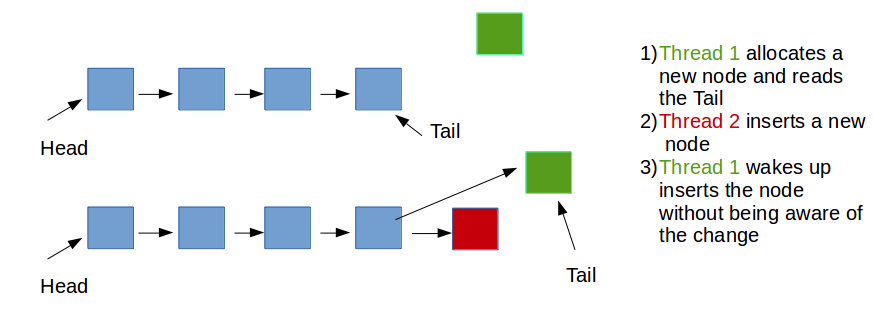
\includegraphics[scale=0.5]{queue_no_sync.png}
\caption{An example of how lack of proper synchronization can make a queue inconsistent}
\label{queue_no_sync}
\end{figure}

Given the low level parallelization offered by the structure, the problem of high performance, essentially becomes the problem of finding a low cost synchronization scheme, as well as achieving better cache utilization.

\subsection{Global Lock}
In our first implementation we adopted a naive, coarse grained strategy. We introduce a global lock, which every thread is trying to set at the beginning of an enqueue or a dequeue. As expected,  performance shown in figure\ref{queue_global_lock_perf} is disappointing and the implementation does not scale. Since only one thread can execute an operation on the structure every given time, while all the other threads spin on the lock, we would expect performance to remain unchanged for any given number of threads. Instead, we can see an imediate and rapid decrease in throughput. %The amount of work done in the critical section is so small that the overhead of synchronization over the lock becomes dominant instantly.

\begin{figure}
 \centering
  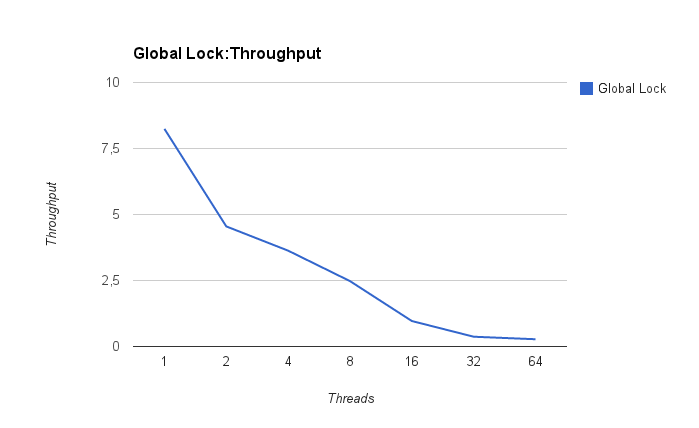
\includegraphics[scale=0.7]{queue_global_lock_perf.png}
\caption{Performance of the naive global lock approach}
\label{queue_global_lock_perf}
\end{figure}


The reason for this poor performance is that the naive global lock implementation cause heavy cache coherence protocol traffic and bus congestion. Even after we implemented and used a TTAS( Test and Test And Set) lock that reduces traffic due to the cache coherence protocol, delays were still high. The main reason is that constantly reading the lock to check it's state produces heavy traffic. Also, since the lock is changing owners frequently, pointers on the list will ping pong back and forth across different caches, causing a lot of cache misses. 

\begin{figure}
 \centering
  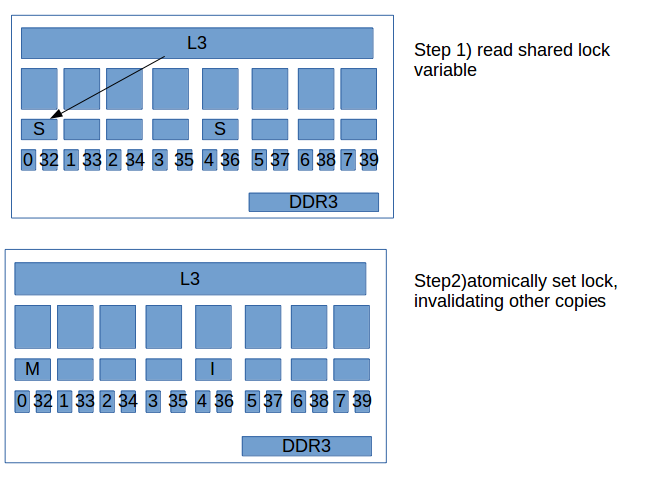
\includegraphics[scale=0.5]{sandman_ping_pong_1.png}
%\caption{Cache coherence traffic on the simple lock queue}
\label{sandman_ping_pong_1}
\end{figure}
\begin{figure}
 \centering
  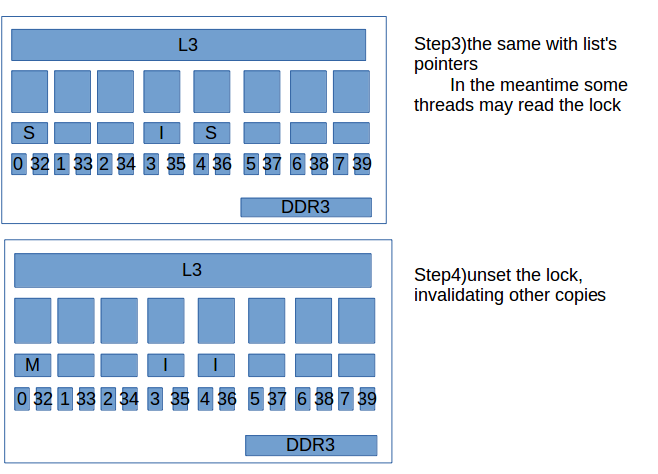
\includegraphics[scale=0.5]{sandman_ping_pong_2.png}
\caption{Cache coherence traffic on the simple lock queue}
\label{sandman_ping_pong_2}
\end{figure}

A solution to that problem is the introduction of backoff: when a thread finds a lock taken, it wont try to check its state again for a while, but will instead wait on loop for a few iterations. This way, the shared memory location is not polled so often,benefiting the general throughput as shown in figures \ref{queue_global_backoff_1} and \ref{queue_global_backoff_2}.


\begin{figure}
 \centering
  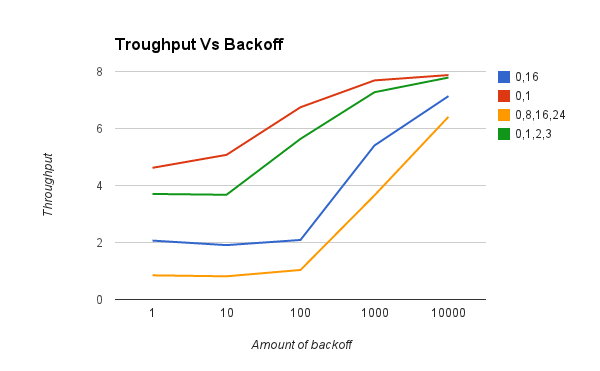
\includegraphics[scale=0.7]{queue_global_backoff_1.png}
\caption{The amount of backoff affects throughput. Points on the horizontal axis are the number of iterations spend waiting on a loop. Red and green lines represent of threads inside the same node, while in blue and yellow lines, threads are placed across multiple nodes}
\label{queue_global_backoff_1}
\end{figure}

\begin{figure}
 \centering
  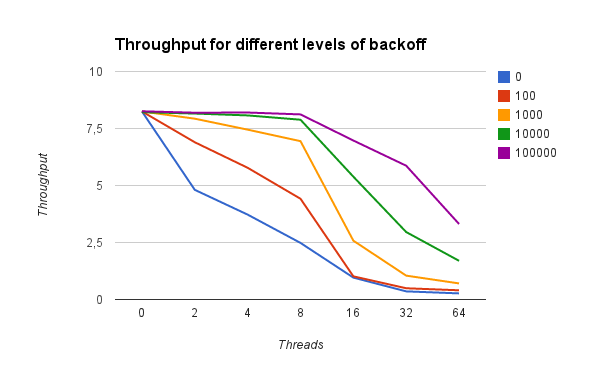
\includegraphics[scale=0.7]{queue_global_backoff_2.png}
\caption{The overall scalling of global lock implementation for various amounts of backoff}
\label{queue_global_backoff_2}
\end{figure}

We can easily see that in general, longer backoff generally increases overall throughput. The reason is more than the reduced traffic caused from polling on the lock. A high backoff means that threads that not manage to take the lock will become inactive for a while, but the thread that takes the lock will quickly complete the critical section (which is very small) and will probably return to attempt another operation very soon. At that time, the other threads will be inactive, spending time backing off, and that thread will probably take the lock again, hitting L1 cache for the memory location of the lock, the Head and the Tail. This certainly improves performance by reducing cache misses, but makes the lock quite unfair: a thread that finds a lock taken may have to wait a long time before setting it to perform a single operation, while a thread that takes the lock will probably retake it several times in a row.   

Another characteristic behavior is that throughput declines dramatically when the number of parallel threads exceeds the number of available cores. In this case, more than one threads share the same core and if a thread holding the lock is scheduled out, no other thread is advancing until that threads regains the CPU and unsets the lock. This is a general problem with locking implementations: If a thread inside the critical section is delayed, the progress of all other threads is halted and performance suffers significantly, making blocking algorithms not suitable for real-time applications.


For this reason, in the field of data structures in general and FIFO Queues in particular, great effort has been applied to come up with efficient, lock free implementations. One of the first, well known, successful implementation of a lock-free FIFO Queue is from Michael and Scott \cite{msqueue} and it serves as a base line for all further efforts.

\section{Michael Scott Queue}
\subsection{Description}

In the Michael Scott approach the data structure is implemented as a simply linked list, with a pointer Head referencing the start of the list, where dequeues are applied and a pointer Tail at the end where we can add new nodes. The node pointed by Head is considered a dummy node  and is used to ensure that the list is never left empty.

In its core, the algorithm uses atomic operations ( in particular Compare And Swap operations) to atomically modify the appropriate pointers. Every time, we run checks to make sure that we have a consistent view of the pointers we are trying to modify.

As depicted in figure \ref{ms_queue_struct}, an enqueue requires 2 atomic operations: one to link the last node with the new node we are trying to insert and one to swap the Tail pointer to the new node.

% εικόνα 1 από το optimistic paper
\begin{figure}
 \centering
  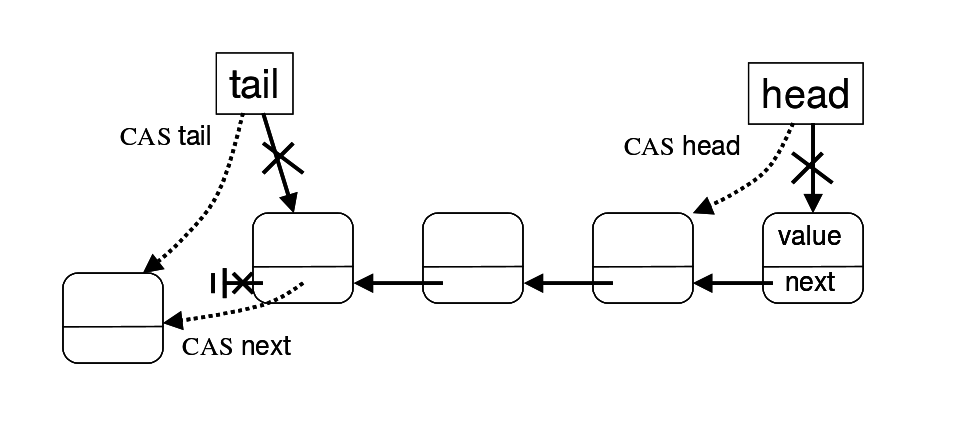
\includegraphics[scale=0.4]{msqueue_struct.png}
\caption{ The basic layout of the link list used in Michael Scott implementation}
\label{ms_queue_struct}
\end{figure}

On the other hand, we need only one C-A-S on the value of Head to perform a dequeue.

\subsection{Challenges}
At any given time during the execution of a thread, the values of Head and Tail can change unexpectedly, causing the atomic operations to fail and the execution to start over from the top: read the new value of Head/Tail and try to change it atomically. Moreover, in order for an enqueue to finish, both two required C-A-Ss need to succeed. This in turn makes it possible for the new node to be added to the list, without updating the value of Tail accordingly, i.e. Tail doesn't point to the last node. For  this reason, during enqueue or dequeue, it is necessary to check for this inconsistency and correct it.

%One of the problems that occurs during the implementation of this algorithm in particular and of algorithms that use C-A-S in general, is the so called ABA problem. In summary, the problem is described by the following scenario: A process observes that a memory location is in a state A and then is halted for a while. In the meantime, another process alters the state of the memory location to B, then back to A again. The initial process will find that the state of the memory location is A and a CAS will succeed, without knowing that the state has changed in the meantime. This problem is related to the lack of a garbage collector that would ensure that we could not release a memory segment that is still being referenced by a thread.

In order to solve the ABA problem, we chose to use modification counters, which we increase on every successful C-A-S and we incorporate them along with every pointer on the data structure. Atomic operations are now performed, not on the pointer but on the pair \textless pointer, modification counter\textgreater which is now treated as a single variable. Thus, we now have to treat pointers in a non traditional way, extracting them from the variable using bit shifting which causes overheads and make programming more difficult and error prone. 

%Alternatively,  there have been put forward many ways to solve the ABA problem, for example with the use of reference counters, that doesn't require merging counters and pointers.

The basic outline of the algorithm is shown bellow:

\begin{lstlisting}

void enqueue (Queue_t * Q , int value){
	
	node = allocate new node
	node->value = value
	node->next.ptr = NULL
	while (1){
		tail = Q->Tail
		next = tail.ptr->next
		if tail == Q->Tail
			if next.ptr == NULL
				if CAS(&tail.ptr->next,next, <node, next.count+1>)
					break
			else
				CAS(&Q->Tail, tail, <next.ptr, tail.count+1>)  
	}				
	CAS(&Q->Tail, tail <node, tail.count+1>)	
}

boolean dequeue (Queue_t *Q, int * pvalue){
	
	while (1){
		head = Q->Head
		tail = Q->Tail
		next = head->next
		if head == Q->Head
			if head.ptr == tail.ptr
				if next.ptr == NULL
					return False
				CAS(&Q->Tail, tail, <next.ptr, tail.count+1>)
			else
				*pvalue= next.ptr->value
				if CAS(&Q->head, head, <next.ptr, head.count+1>)
					break
	}
	free(head.ptr)
	return True
}

\end{lstlisting}

\begin{figure}
 \centering
  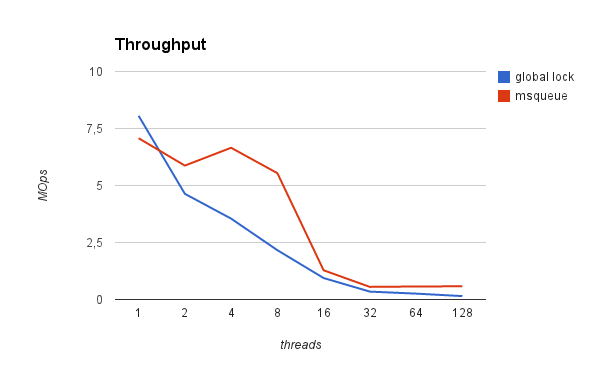
\includegraphics[scale=0.7]{queue_msqueue_perf.png}
 \caption{ Performance of the Michael Scott queue compared to the global lock queue}
\label{queue_msqueue_perf}
\end{figure}

The result is a lock-free implementation,  that does not require central locking of the data structure and allows all threads to advance. The absence of a lock leaves us with one less, heavily contested shared memory location to worry about. Performance is not affected by random delays that a thread can have, achieving robustness. Especially during over subscription, performance does not degrade like global locks' does.

On the other hand, CAS operations have a substantial cost, greater than a simple store. This store is even greater when the atomic operation is performed over different NUMA node, hence the sudden drop in performance when threads leave the package. Moreover, failing a CAS means that the operation needs to start over, stalling this particular thread, while others progress.  

\begin{figure}
 \centering
  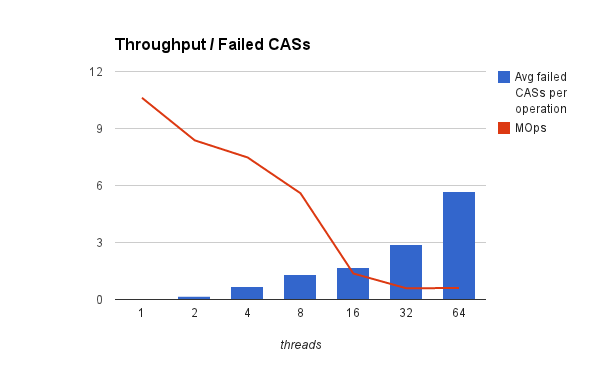
\includegraphics[scale=0.7]{queue_msqueue_CAS_contention.png}
 \caption{ Performance and number of CASs per operation}
\label{queue_msqueue_CAS_contention}
\end{figure}

The number of CASs needed to perform an operation increases with contention, as shown in figure \ref{queue_msqueue_CAS_contention}. Again, we try to reduce contention by introducing backoff after a threads fails to perform a CAS. The results shown in figure \ref{queue_msqueue_backoff} suggest a modern amount of speedup, once again, at the expense of fairness. 

\begin{figure}
 \centering
  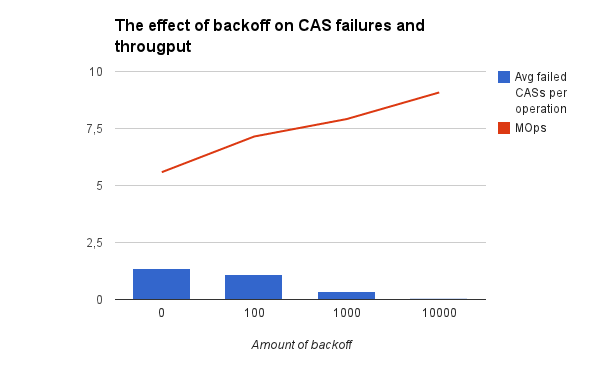
\includegraphics[scale=0.7]{queue_msqueue_backoff.png}
 \caption{ The effects of backoff on the performance of the Michael Scott Queue}
\label{queue_msqueue_backoff}
\end{figure}


\section{Optimistic Queue}

\subsection{introduction}
One of the drawbacks of lock-free approaches is that, each time an atomic operation fails, the execution start back from the top. Moreover, failed atomic operations are costly, due to the synchronization barrier they introduce. Especially in Michael Scott Queue, since both two atomic operations need to be successful in order to complete an enqueue, it is quite common for a thread to repeat execution again and again until it is done correctly. For this reason, we would like to reduce the number of synchronization points ,i.e. the number of atomic operations.

A solution to this problem is introduced by the next algorithm we implemented, by Ladan-Mozes and Shavit \cite{optimistic}. This implementation follows an optimistic approach ( which is why we will refer to this implementation as optimistic queue), in a sense that it runs quickly on the common case where there is no conflict and leaves the costly operations for the case where an inconsistency is spotted. In particular, one of the two C-A-S operations, during enqueue, is replaced with a simple local store, making sure that we correct the data structure in case it is inconsistent.

\subsection{implementation}
Practically, the link list becomes a doubly linked list, with the "next" directions being from Tail to Head. In this way, we only need a single C-A-S to Tail to make it point to the new node, in order to successfully complete an enqueue. However, in order to have access to node from head when we dequeue, we need pointers in the reverse order, as seen in figure \ref{optimistic_struct}.

%figure 2 apo optimistic paper
\begin{figure}
 \centering
  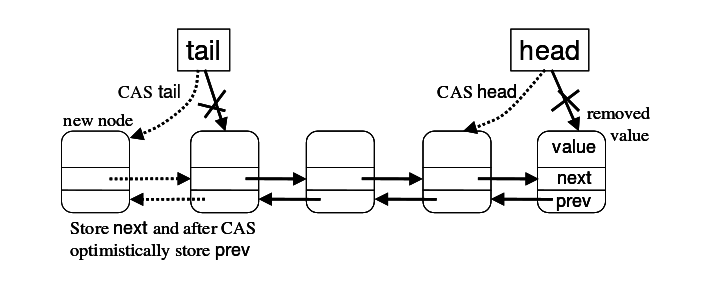
\includegraphics[scale=0.6]{optimistic_struct.png}
 \caption{ The basic layout of the doubly linked list used in the Optimistic Queue}
\label{optimistic_struct}
\end{figure}

Pointers in both directions are updated with simple local stores , without synchronization, which makes inconsistencies possible, in the "prev" direction. For this reason, as soon as an inconsistency is spotted, function FixList is called to traverse the list and fix all the pointers. However, the reason for inconsistencies in the "prev" direction are the long delays a single thread might take and not contention. Therefore, we expect the number of calls to FixList to remain low, even when the number of parallel threads increases.

Inserting a new node in the list includes 3 steps:
1) Set the next pointer of the new node we are trying to insert
2) Compare And Swap on Tail, to make it point to the new node
3) Change the prev pointer of the next node.

\begin{lstlisting}
void enqueue ( Queue_t * Q, int value){
	
	node = allocate new node
	node->value = val
	while (1){
		tail = Q->tail
		node->next = <tail.ptr, tail.tag +1>
		if CAS(&(Q->Tail), tail, <node, tail.tag+1>)
			(tail.ptr)->prev = <node, tail.tag>
			break
	}

}

\end{lstlisting}
\subsection{ABA and consistency}

In order to avoid the ABA problem and spot inconsistencies, this implementation also uses modification counters, that are merged along with the pointers and are incremented in every successful C-A-S

Any thread might take arbitrary time  between steps 2 and 3 and during this time more nodes might be inserted in the queue. Note however that, every time a node is successfully inserted in the queue(after successful C-A-S), the modification counter to be inserted next is incremented by one. Thus, pointers of consecutive nodes in the queue, will have consecutive modification counters. In this way, during a dequeue, if a prev pointer does not have the expected modification counter, FixList is called and the pointers are repaired.

\begin{lstlisting}
void fixList(Queue_t Q, tail, head){
	curNode = tail
	while((head == Q->Head) && (curNode != head){
		curNodeNext = (curNode.ptr)->next
		if (currNodeNext.tag != curNode.tag)
			return
		
		nextNodePrev = (curNodeNext.ptr)->prev
		if (nextNodePrev != <curNode.ptr, curNode.tag - 1>)
			(curNodeNext.ptr)->prev = <currNode.ptr, currNode.tag -1>
		
		curNode = <curNodeNext.ptr, curNode.tag -1 >
	}
}
\end{lstlisting}

Note that there must be special care taken to ensure that there is always one dummy node in the list and Tail never goes past that node.

\subsection{Failed C-A-S operations}

The next diagram compares the number of C-A-S operations( both successful and failed) needed to execute 1 million pairs of enqueue/dequeue, across these two lock-free implementations. We can see that the optimistic approach, as promised, requires less C-A-Ss and has, in total less costly, failed C-A-Ss as the level of concurrency increases.

%διαγραμμα για failed CAS
\begin{figure}
 \centering
  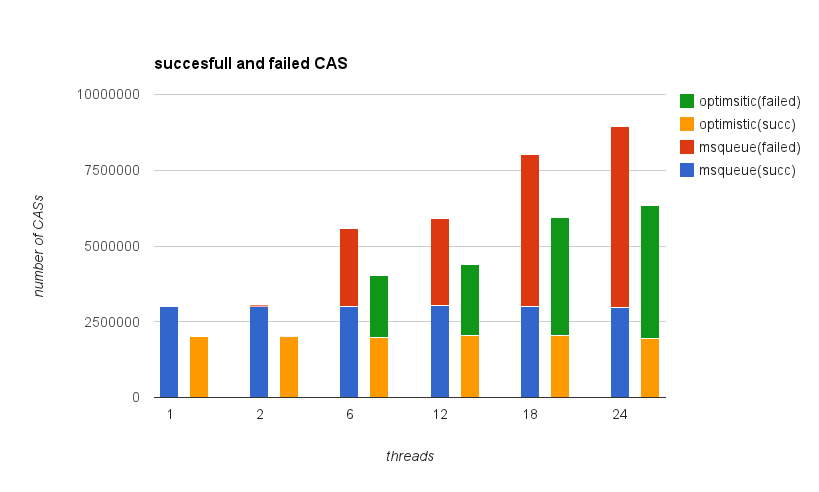
\includegraphics[scale=0.5]{failed_cas.png}
\caption{Total successful and failed C-A-Ss for the two lock-free implementations}
\end{figure}

We can see in figure \ref{queues_oversubscription} that during over-subscription, the global lock's performance suffers whereas lock-free approaches do not seem to be affected, since they are more robust against preemptions.


\begin{figure}
 \centering
  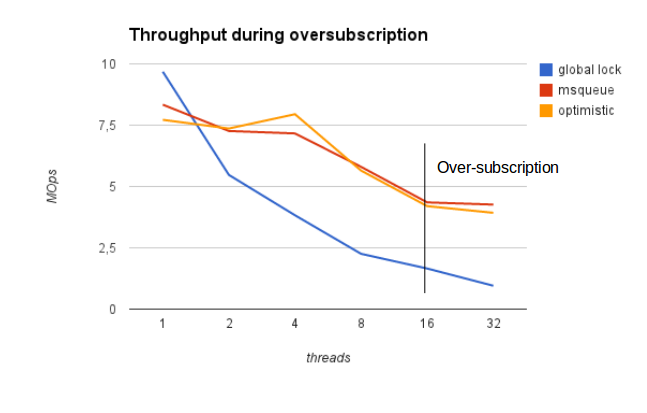
\includegraphics[scale=0.5]{queues_oversubscription.png}
\caption{The effects of over-subscription on locking and lock free algorithms}
\label{queues_oversubscription}
\end{figure}

All in all, the optimistic optimization seems to contribute a slight amount of speedup, compared to the Michael Scott queue, as shown in figure \ref{queue_optimistic_perf}. The overall performance of the concurrent queue has significantly increased since the naive global lock algorithm, but many problems still remain. The very small critical section makes synchronization a high fraction of the total cost. Adding backoff was a step forward but it would potentially introduce heavy overheads for some threads.


\begin{figure}
 \centering
  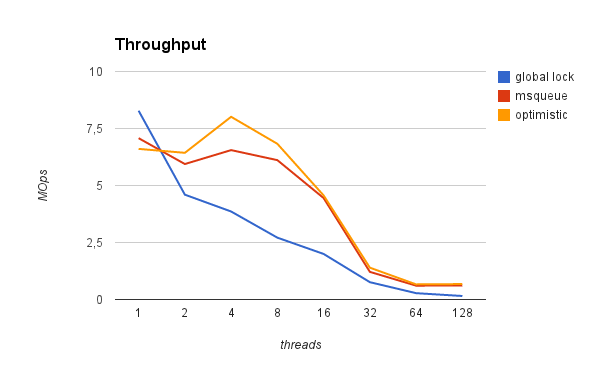
\includegraphics[scale=0.5]{queue_optimistic_perf.png}
\caption{The performance of the optimistic approach}
\label{queue_optimistic_perf}
\end{figure}

\section{Flat Combining}
\subsection{Introduction}

The two previous implementations followed a fine grain approach, where every thread has access to the data structure and they are trying to achieve performance through high parallelization. As more treads are free to operate on the data structure, performance is expected to be better that locking approaches that block the progress of some threads. We next present the principles of flat combining, a programming approach by Hendler, Incxe and Shavit \cite{flat_combining} that goes against the above mentioned statements.

In particular, the authors claim that the point at which the cost of synchronization between threads exceeds the benefit from high parallelization, is at a lower lever of concurrency than expected. Flat combining is based on a synchronization scheme where each thread locks  the data structure in an extremely low-cost way, gathers information on the operations trying to be executed on the queue by the other threads and then does the operations in their place. The result is an implementation with low synchronization cost and better cache performance, overcoming the drawbacks of blocking and low parallelization.

\subsection{Implementation}

Flat combining is a layer of abstraction that can be used over a sequential structure and its basic functions is the following:
1) Every thread publishes the operations it is trying to perform on the structure, along with any parameters, on its corresponding public record. These records can be in an array, for fast read/write or in linked list with dynamic size, proportional to the number of active threads.
2) Every thread checks the state of the locks and if it finds it unlocked, it tries only once to atomically set the lock. If the lock was locked already, the thread spins in its public record, waiting for a response.
3) If it takes the lock, this thread is considered the new combiner. It then traverses the public records and executes the request on the data structure, one by one, writing back the results. Finally the thread releases the lock.


\begin{figure}
 \centering
  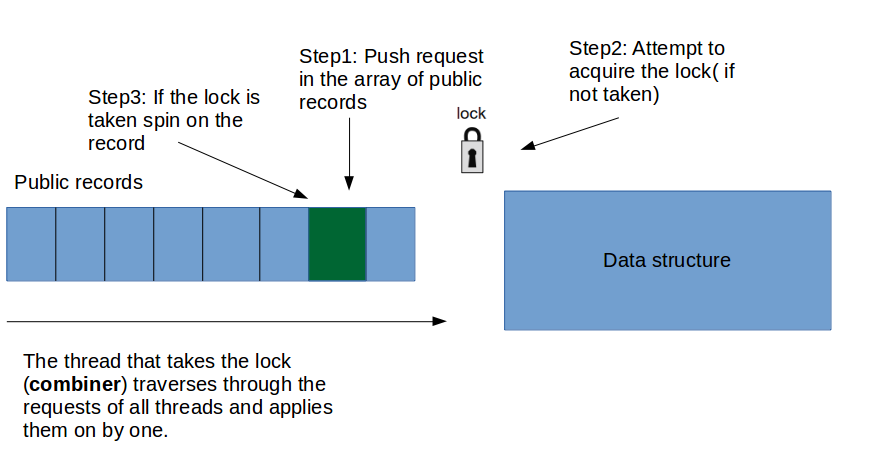
\includegraphics[scale=0.5]{flat_combining_basic.png}
\caption{The basic synchronization scheme of flat combining}
\label{flat_combining_basic}
\end{figure}

The definition of the public record structure, as well as the main steps take by every thread are shown bellow:

\begin{lstlisting}

struct pub_record{
	int pending
	int operation
	int value
	int response
} 

int try_access(Queue_t Q, struct pub_record * pub, int operation, int value){
	int thread_id
	pub[thread_id].operation = operation
	pub[thread_id].value = value
	pub[thread_id].pending = 1
	while (1){
		if ( Q->lock){

			while (!pub[thread_id].response) do nothing
			
			pub[tid].response = 0
			return pub[tid].value
		}
		else{
			if (__sync_lock_test_and_set(&(Q->lock), 1)) 
				continue;
			else{
				for i=0 to number of threads
					if pub[i].pending{
						if pub[i].op ==1
							do the actual enqueue
						else
							do the actual dequeue
						pub[i].pending=0
						pub[i].response=1
					}
				}
				
				pub[thread_id].response=0
				Q->lock = 0
				return pub[thread_id].value
		}
	}
}				

\end{lstlisting}
% isws kana sxhmataki  gia th domh  san auto sto paper

\subsection{Implementation characteristics and Benefits}
From the way flat combining works, certain advantages can be concluded:
1)Since only the combiner has access to the structure, operations can be optimized with the best sequential algorithm, without minding synchronization and concurrency. This even allows us to implement concurrent structures, such as pairing heaps, that are otherwise difficult to implement using fine grain synchronization, by applying flat combining over already existent sequential data structures.
2) in some cases, the combiner can use some smart way to group the request and make the access to the structure faster and more efficient. For example, in concurrent stacks, a combiner can perform elimination between a concurrent enqueue and a concurrent dequeue. In our queue implementation, we used fat nodes to group data, as we explain later on.
3) The combined way of accessing the structure by a single thread can lead to better cache utilization.
4) Using a global lock to isolate the structure makes programming, as well as debugging, much easier.

It is also important to note that flat combining, as a layer of abstraction that ensures synchronization, can bee used as it is over different data structured. Of course, not all data structures are benefited by flat combining. For example, if the cost of a single operation in a search tree is \textgreek{Θ} (logn), using flat combining, the cost of k operations is in general \textgreek{Θ} (klogn), while we could  use parallel threads that execute operations independently on different parts of the tree in \textgreek{Θ} (longn) total time.

FIFO Queues in particular, seem to benefit by flat combining, given that they already allow low levels of concurrency ( only two access points). In our implementation, we organized public records in an array and used fat nodes, where every node can hold up to 16 values. Therefore, we only need to add one node in the queue and swap the Tail pointer only once, for every 16 values inserted. We also used two independent instances of flat combining, one for enqueues and one for dequeues, in order to exploit the maximum concurrency allowed.

\subsection{First results}
 
\begin{figure}
 \centering
  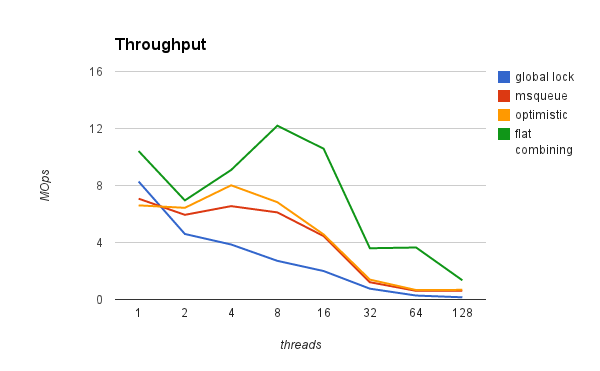
\includegraphics[scale=0.7]{queue_fc_queue_perf.png}
\caption{Perfromance of flat combining, compared to the other approaches}
\label{queue_fc_queue_perf}
\end{figure}

Figure \ref{queue_fc_queue_perf} shows the overall performance of flat combining compared to the other approaches. Performance seems to benefit greatly from the way batches of work are done by a single thread and the light-weight synchronization scheme. Especially inside the node, a fairly good scaling is noted. Trying to utilize that benefit even more, we keep the combiner iterating over the the public records more than once. Figure \ref{queue_fc_queue_loops} shows that assigning more work to every combiner, although harmful when only a few threads are utilized, offers a slight speedup when more than 4 threads are used. Note however that this further increases the potential latency of the thread that becomes a combiner. 


\begin{figure}
 \centering
  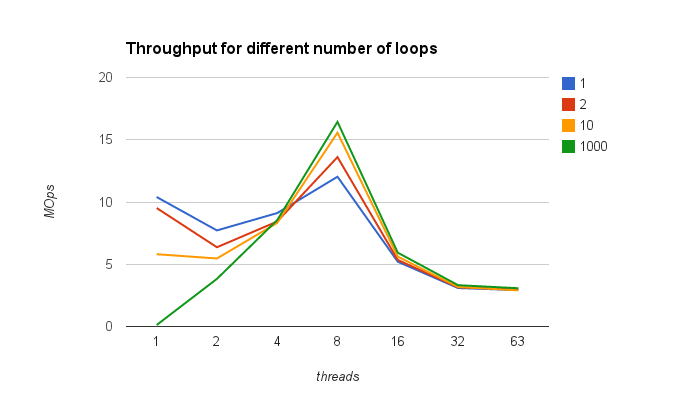
\includegraphics[scale=0.7]{queue_fc_queue_loops.png}
\caption{The effects of keeping the combiner iterating more than once over the public records}
\label{queue_fc_queue_loops}
\end{figure}

\subsection{Optimizations}
%1 dedicated combiner


From the analysis of the algorithm we can deduct that every thread can, in theory, access the queue and alter its state. That means that the nodes of the queue can be in the cache memory of any thread, which in turn leads to increased cache misses and long delays.

By extending that idea, we can see that it might be better to have a dedicated combiner, residing in a specific core that will serve all requests. This way references on the lists nodes will always hit


The result, shown in figure \ref{queue_fc_dedicated_perf}, is a constant improvement in performance, that corresponds  to less cache misses and better locality. Again, however, leaving the package significantly degrades performance and in fact, the overhead of communication between packages quickly becomes the dominant cost.

\begin{figure}
 \centering
  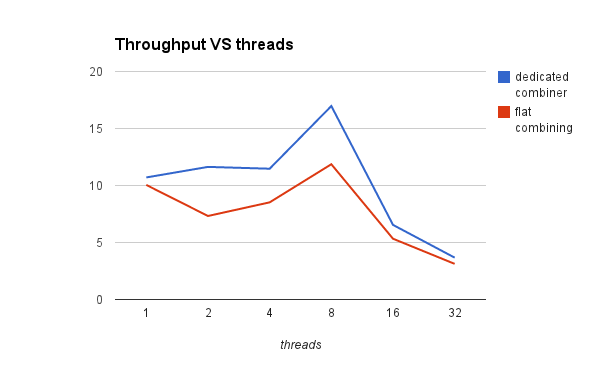
\includegraphics[scale=0.7]{queue_fc_dedicated_perf.png}
\caption{The speed up achieved by using a dedicated combiner}
\label{queue_fc_dedicated_perf}
\end{figure}

Addressing that problem,we can see that the flat combining synchronization scheme, as it is, introduces a lot of communication over different nodes, as the combiners need to read and modify the publication record of a thread that is on a different package.


The previously implemented flat combining algorithm is not NUMA-aware and cannot deal with the problems mentioned above. For this reason, we designed and implemented a hybrid implementation that combines previous algorithms, taking architecture into account, in order to achieve better performance.

The implementation that was eventually chosen  consists of two stages. In the first stage, we use flat combining in every NUMA node. Threads of the same node are synchronized to come up with a combiner. In the second stage, combiners from each node are further synchronized to access the queue. In the second stage we tried several synchronization schemes ( Michael-Scott queue, a second level of flat combining). Eventually, the best performance for the given architecture was achieved by a simple TTAS global lock.

\begin{figure}
 \centering
  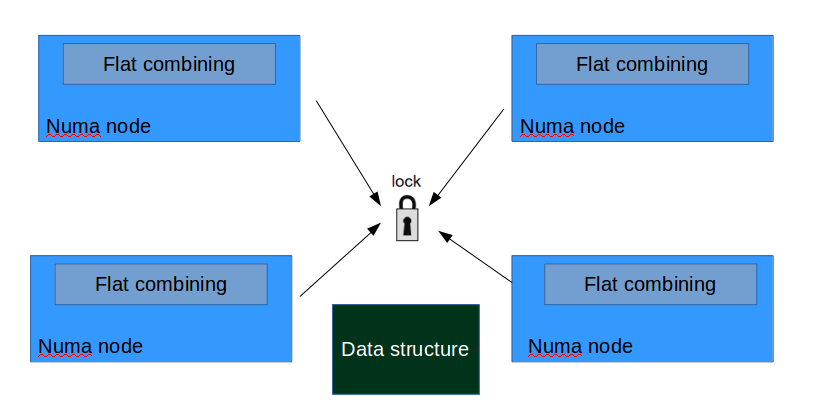
\includegraphics[scale=0.5]{queue_fc_hybrid_basic.png}
\caption{The use basic layout of the hybrid aproach}
\label{queue_fc_hybrid_basic}
\end{figure}

The result was a limited improvement of the performance when threads reside across several nodes, shown in figure \ref{queue_fc_hybrid_perf}.

 
\begin{figure}
 \centering
  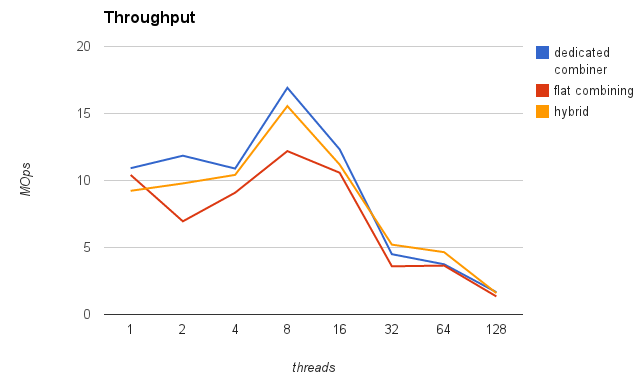
\includegraphics[scale=0.7]{queue_fc_hybrid_perf.png}
\caption{The use performance of the hybrid aproach compared to other flat combining schemes}
\label{queue_fc_hybrid_perf}
\end{figure}

